\subsection{Integration Techniques}
\subsubsection{Substitution}
Substitution is used to help solve messy integrals and is a very common tool. It is the opposite to the chain rule. We can choose an expression of $x$ to replace with $u$. Note that this will also change the differential and the bounds of integration.
\begin{align*}
    \text{Ex: }&\int (x+2)^{10}dx\\
    &\text{let }u=x+2\Ra du=dx\\
    &\int u^{10}du=\frac{u^{11}}{11}+C\\
    &=\frac{(x+2)^{11}}{11}+C
\end{align*}
\begin{align*}
    \text{Ex2: }&\int(5x^2+1)\sqrt{5x^3+3x-2}dx\\
    &\text{let }u=5x^3+3x-2\\
    &du=(15x^2+3)dx\Ra\frac{du}{3}=(5x^2+1)dx\\
    &\int \frac{1}{3}\sqrt{u}du=\frac{1}{3}\frac{u^{3/2}}{3/2}+C=\frac{2u^{3/2}}{9}+C\\
    &=\frac{2}{9}(5x^3+3x-2)^{3/2}+C
\end{align*}
\begin{align*}
    \text{Ex3: }&\int \frac{\sin x}{(2+\cos x)^2}dx\\
    &\text{let }u=2+\cos x\\
    &du=-\sin x dx\Ra-du=\sin x dx\\
    &\int\frac{-du}{u^2}=\frac{1}{u}+C\\
    &=\frac{1}{2+\cos x}+C
\end{align*}
\begin{align*}
    \text{Ex4: }&\int\frac{\ln x}{x}dx\\
    &\text{let }u=\ln x\Ra du=\frac{dx}{x}\\
    &\int udu=\frac{u^2}{2}\\
    &=\frac{(\ln x)^2}{2}+C
\end{align*}
\begin{align*}
    \text{Ex5: }&\int a^xdx\\
    &a^x=e^{\ln a^x}=e^{x\ln a}\\
    &\text{let }u=x\ln a\Ra du=\ln a\\
    &\int \frac{e^{u}}{\ln a}du=\frac{e^u}{\ln a}+C=\frac{e^{x\ln a}}{\ln a}+C\\
    &=\frac{a^x}{\ln a}+C
\end{align*}
\begin{align*}
    \text{Ex6: }&\int\tan xdx\\
    &I=\int\frac{\sin x}{\cos x}dx\\
    &\text{let }u=\cos x\Ra du=-\sin xdx\Ra -du=\sin xdx\\
    &I=-\int\frac{du}{u}=-\ln|u|+C\\
    &=-\ln|\cos x|+C
\end{align*}
Note that when we use substitution with a definite integral, the bounds change.
\begin{align*}
    \text{Ex7: }&\int_0^1\frac{3x}{(x^2+1)^2}dx\\
    &\text{let }u=x^2+1\Ra du=2xdx\Ra \frac{3}{2}du=3dx\\
    &u(0)=1,\,u(1)=2\\
    &I=\frac{3}{2}\int_1^2\frac{du}{u^2}=\frac{3}{2}\brsquare{-\frac{1}{u}}^2_1\\
    &=\frac{3}{4}
\end{align*}
\subsubsection{Integration by Parts}
Integration by parts is the opposite of the product rule.
\begin{align*}
    &d(uv)=udv+vdu\\
    &udv=d(uv)-vdu\\
    &\int udv=uv-\int vdu
\end{align*}
Using the derived formula, we can decompose the integral of a product in the following way.\\
Typically, we take $u$ to be a function easy to differentiate and $dv$ to be a function easy to integrate.
\begin{align*}
    \text{Ex: }&\int x\sin xdx\\
    &\text{let }u=x\Ra du=dx\\
    &\text{let }dv=\sin xdx\Ra v=-\cos x\text{*}\\
    &\int x\sin xdx=-x\cos x+\int \cos xdx\\
    &=-x\cos x+\sin x+C
\end{align*}
*Note we ignore the $+C$ when integrating $dv$ as we instead add it in later with the final solution.\\
Sometimes, we may have to complete integration by parts multiple times to get a solution.\\
Other times, we may never be able to solve explicitly but can come to an answer by recursion.
\begin{align*}
    \text{Ex2: }&I=\int e^{2x}\cos x dx\\
    &\text{let }u=e^{2x}\Ra du=2e^{2x}dx\\
    &\text{let }dv=\cos xdx\Ra v=\sin x\\
    &I=e^{2x}\sin x-\int \sin x2e^{2x}dx=e^{2x}\sin x-2\int e^{2x}\sin x dx\\
    &\text{solve }\int e^{2x}\sin xdx\\
    &\text{let }u=e^{2x}\Ra du=2e^{2x}dx\\
    &\text{let }dv=\sin xdx\Ra v=-\cos x\\
    &I=e^{2x}\sin x-2\brround{-e^{2x}\cos x-\int (-\cos x)(2e^{2x}dx)}\\
    &I=e^{2x}\sin x+2e^{2x}\cos x-4\int e^{2x}\cos xdx\\
    &\text{recall }I=\int e^{2x}\cos x dx\\
    &I=e^{2x}\sin x+2e^{2x}\cos x-4I\\
    &5I=e^{2x}\sin x+2e^{2x}\cos x\\
    &I=\frac{1}{5}\brround{e^{2x}\sin x+2e^{2x}\cos x}+C
\end{align*}
\begin{align*}
    \text{Ex3: }&\int \ln xdx\\
    &\text{let }u=\ln x\Ra du=\frac{dx}{x}\\
    &dv=dx\Ra v=x\\
    &I=x\ln x-\int \frac{x}{x}dx\\
    &=x\ln x-x+C
\end{align*}
\begin{align*}
    \text{Ex4: }&\int \arctan xdx\\
    &\text{let }u=\arctan x\Ra du=\frac{dx}{1+x^2}\\
    &dv=dx\Ra v=x\\
    &I=x\arctan x-\int\frac{x}{1+x^2}dx\\
    &\text{let }w=1+x^2\Ra dw=2dx\Ra \frac{dw}{2}=dx\\
    &I=x\arctan x-\frac{1}{2}\int\frac{dw}{w}=x\arctan x-\frac{1}{2}\ln w+C\\
    &=x\arctan x-\frac{1}{2}\ln(1+x^2)+C
\end{align*}
Ex5: Let $I_n=\int_0^{2\pi}\sin^n xdx$. Determine a recursive relation for $I_n$ and compute $\int_0^{2\pi}\sin^6xdx$
\begin{align*}
    &I_n=\int_0^{2\pi}\sin^{n-1}x\sin xdx\\
    &u=\sin^{n-1}x\Ra du=(n-1)\sin^{n-2}x\cos x dx\\
    &dv=\sin xdx\Ra v=-\cos x\\
    &I_n={-\sin^{n-1}x\cos x}\eval_0^{2\pi}+(n-1)\int_0^{2\pi}\sin^{n-2}x\cos^2xdx\\
    &I_n=0+(n-1)\int_0^{2\pi}(1-\sin^2x)\sin^{n-2}xdx\\
    &I_n=(n-1)\int_0^{2\pi}\sin^{n-2}xdx-(n-1)\int_0^{2\pi}\sin^nxdx\\
    &I_n=(n-1)I_{n-2}-(n-1)I_n\\
    &I_n=\frac{n-1}{n}I_{n-2}\\
    &\text{So, }\int_0^{2\pi}\sin^6xdx=I_6=\frac{5}{6}I_4=\frac{5}{6}\cdot\frac{3}{4}I_2=\frac{5}{6}\cdot \frac{3}{4}\cdot\frac{1}{2}I_0\\
    &I_0=\int_0^{2\pi}dx=2\pi\\
    &\therefore I_6=\frac{5\pi}{8}
\end{align*}
\subsubsection{Trigonometric Integrals}
Integrals of products of sines and cosines:\\
$\int\sin^ax\cos^bxdx$ where $a$ and $b$ are intigers.\\
Case when $a$ is odd:
\begin{align*}
    &\int\sin^ax\cos^bxdx=\int\sin^{a-1}x\cos^bx\sin xdx=\int(1-\cos^2x)^{\frac{a-1}{2}}\cos^bx\sin xdx\\
    &u=\cos x\Ra -du=\sin xdx\\
    &I=-\int u^b(1-u^2)^{\frac{a-1}{2}}du
\end{align*}
\begin{align*}
    \text{Ex: }&\sin^3x\cos^3xdx\\
    &\int(1-\cos^2x)\cos^3x\sin xdx\\
    &u=\cos x\Ra -du=\sin x\\
    &I=-\int(1-u^2)u^3du=-\int(u^3-u^5)du\\
    &I=\frac{u^6}{6}-\frac{u^4}{4}+C\\
    &=\frac{\cos^6x}{6}-\frac{\cos^4x}{4}+C
\end{align*}
Case when $b$ is odd:
\begin{align*}
    &\int sin^ax\cos^bxdx=\int\sin^ax\cos^{b-1}x\cos xdx=\int\sin^ax(1-\sin^2 x)^{\frac{b-1}{2}}\cos xdx\\
    &u=\sin x\Ra du=\cos xdx\\
    &I=\int u^a(1-u^2)^\frac{b-1}{2}du
\end{align*}
\begin{align*}
    \text{Ex: }&\int\sin^2x\cos^5xdx\\
    &I=\int\sin^2x(1-\sin^2x)^2\cos xdx\\
    &u=\sin x\Ra du=\cos xdx\\
    &I=\int u^2(1-u^2)^2du=\int(u^2-2u^4+u^6)du\\
    &I=\frac{u^3}{3}-\frac{2u^5}{5}+\frac{u^7}{7}+C\\
    &=\frac{\sin^3 x}{3}-\frac{2\sin^5x}{5}+\frac{\sin^7x}{7}+C
\end{align*}
Case when $a$ and $b$ are even:\\
In this case, we will require the following half-angle identities
\begin{align*}
    \cos(2\theta)&=\cos^2\theta-\sin^2\theta\\
    &=\cos^2\theta-(1-\cos^2\theta)\\
    &=2\cos^2\theta-1\\
    &\Ra\cos^2\theta=\frac{1+\cos(2\theta)}{2}
\end{align*}
We also have that
\begin{align*}
    \sin^2\theta=\frac{1-\cos(2\theta)}{2}\\
\end{align*}
The goal here is to express the integrand as a single trig term.
\begin{align*}
    \text{Ex: }&\int\sin^2(4x)\cos^2(4x)dx\\
    &I=\int(\sin(4x)\cos(4x))^2dx=\int\brround{\frac{\sin(8x)}{2}}^2dx=\frac{1}{4}\int\brround{\frac{1-\cos(16x)}{2}}dx\\
    &=\frac{1}{4}\brround{\frac{x}{2}-\frac{\sin(16x)}{32}}+C
\end{align*}
Integrals of products of tan and sec:\\
$\int\tan^ax\sec^bxdx$ where $a$ and $b$ are integers.\\
Case when $b$ is even:
\begin{align*}
    &\int\tan^ax\sec^bxdx=\int\tan^ax\sec^{b-2}x\sec^2xdx=\int\tan^ax(1+\tan^2x)^{\frac{b-2}{2}}\sec^2xdx\\
    &u=\tan x\Ra du=\sec^2xdx\\
    &I=u^a(1+u^2)^{\frac{b-2}{2}}du
\end{align*}
\begin{align*}
    \text{Ex: }&\int\tan^2x\sec^4xdx\\
    &I=\int\tan^2x\sec^2x\sec^2xdx=\int\tan^2x(1+\tan^2x)\sec^2xdx\\
    &u=\tan x\Ra du=\sec^2xdx\\
    &I=\int u^2(1+u^2)du\\
    &I=\frac{u^3}{3}+\frac{u^5}{5}+C\\
    &I=\frac{\tan^3x}{3}+\frac{\tan^5x}{5}+C
\end{align*}
Case when $a$ is odd and $b\geq 1$
\begin{align*}
    &\int\tan^ax\sec^bxdx=\tan^{a-1}\sec^{b-1}(\sec x\tan x)dx=\int(\sec^2x-1)^{\frac{a-1}{2}}\sec^{b-1}x(\sec x\tan x)dx\\
    &u=\sec x\Ra du=\sec x\tan xdx\\
    &I=(u^2-1)^{\frac{a-1}{2}}u^{b-1}du
\end{align*}
\begin{align*}
    \text{Ex: }&\int\tan^3x\sec^7xdx\\
    &I=\int\tan^2x\sec^6x(\sec x\tan x)dx=\int(\sec^2x-1)\sec^6x(\sec x\tan x)dx\\
    &u=\sec x\Ra du=\sec x\tan x dx\\
    &I=\int(u^2-1)u^6du=\frac{u^9}{9}-\frac{u^7}{7}+C\\
    &=\frac{\sec^9x}{9}-\frac{\sec^7x}{7}+C
\end{align*}
For other cases, there may not be any specific method.
\begin{align*}
    \text{Ex: }&\int\tan^4xdx\\
    &I=\int\tan^2x\tan^2xdx=\int\tan^2x(\sec^2x-1)dx\\
    &I=\int\tan^2x\sec^2xdx-\int\tan^2xdx\\
    &I=\int\tan^2x\sec^2xdx-\int(\sec^2x-1)dx\\
    &u=\tan x\Ra du=\sec^2xdx\\
    &I=\int u^2du-\int du+\int dx\\
    &I=\frac{u^3}{3}-u+x+C\\
    &=\frac{\tan^3x}{3}-\tan x+x+C
\end{align*}
\begin{align*}
    \text{Ex2: }&\int\sec xdx\\
    &I=\int\sec x\brround{\frac{\sec x+\tan x}{\sec x+\tan x}}dx=\int\frac{\sec^2x+\sec x\tan x}{\sec x+\tan x}dx\\
    &u=\sec x+\tan x\Ra du=(\sec x\tan x+\sec^2x)dx\\
    &I=\int\frac{du}{u}=\ln|u|+C\\
    &=\ln|\sec x+\tan x|+C
\end{align*}
\begin{align*}
    \text{Ex3: }&\int\sin(2x)\cos(3x)dx\\
    &\cos(3x)=\cos(2x+x)=\cos(2x)\cos x-\sin (2x)\sin x=4\cos^3x-3\cos x\\
    &\sin(2x)=2\sin x\cos x\\
    &I=\int(2\sin x\cos x)(4\cos^3x-3\cos x)dx\\
    &I=8\int\cos^4x\sin xdx-6\int\cos^2x\sin xdx\\
    &u=\cos x\Ra -du=\sin xdx\\
    &I=6\int u^2du-8\int u^4du=2u^3-\frac{8u^5}{5}+C\\
    &=-\frac{8}{5}\cos^5x+2\cos^3x+C
\end{align*}
\subsubsection{Trigonometric Substitution}
Often times when integrating a function with a square root we can use a trig substitution to simplify the function.\\
\begin{itemize}
    \item For $\sqrt{a^2+x^2}$ use $x=a\tan\theta$ where $\theta\in\brround{-\frac{\pi}{2},\frac{\pi}{2}}$\\
    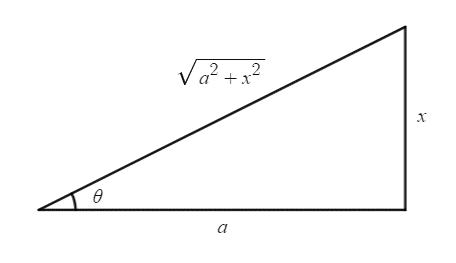
\includegraphics[scale=0.7]{Images/IntegralCalcPictures/TrigSubTan.png}
    \item For $\sqrt{a^2-x^2}$ use $x=a\sin\theta$ where $\theta\in\brsquare{-\frac{\pi}{2},\frac{\pi}{2}}$\\
    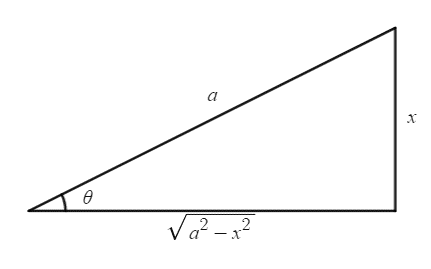
\includegraphics[scale=0.7]{Images/IntegralCalcPictures/TrigSubSin.png}
    \item For $\sqrt{x^2-a^2}$ use $x=a\sec\theta$ where $\theta\in\left[0,\frac{\pi}{2}\right)$\\
    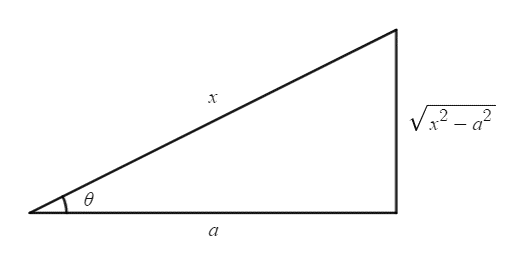
\includegraphics[scale=0.7]{Images/IntegralCalcPictures/TrigSubSec.png}
\end{itemize}
\begin{align*}
    \text{Ex: }&\int \frac{x}{\sqrt{1-x^2}}dx\\
    &x=\sin \theta\Ra dx=\cos\theta d\theta\\
    &\sqrt{1-x^2}=\cos x\\
    &I=\int\frac{\sin\theta\cos\theta}{\cos\theta}d\theta=\int\sin\theta d\theta=-\cos\theta+C\\
    &=-\sqrt{1-x^2}+C
\end{align*}
\begin{align*}
    \text{Ex2: }&\int\frac{dx}{\sqrt{x^2+1}}\\
    &x=\tan\theta\Ra dx=\sec^2\theta d\theta\\
    &\sqrt{x^2+1}=\sec\theta\\
    &I=\int\frac{\sec^2\theta}{\sec\theta}d\theta=\ln|\sec\theta+\tan\theta|+C\\
    &=\ln|x+\sqrt{x^2+1}|+C
\end{align*}
\begin{align*}
    \text{Ex3: }&\int\frac{dx}{x^2\sqrt{x^2-16}}\\
    &x=4\sec\theta\Ra dx=4\sec\theta\tan\theta\\
    &\sqrt{x^2-16}=4\tan\theta\\
    &I=\int\frac{4\sec\theta\tan\theta}{64\sec^2\theta\tan\theta}d\theta=\frac{1}{16}\int\frac{d\theta}{\sec\theta}=\frac{1}{16}\int\cos\theta d\theta\\
    &I=\frac{\sin\theta}{16}+C\\
    &=\frac{\sqrt{x^2-16}}{16x}+C
\end{align*}
Sometimes we may be required to complete the square in order to get the expression under the square root into a form where we can perform a trig substitution
\begin{align*}
    \text{Ex: }&\int\frac{dx}{x^2+4x+7}\\
    &I=\frac{dx}{x^2+4x+4+7-4}=\int\frac{dx}{(x+2)^2+3}\\
    &\frac{x+2}{\sqrt{3}}\tan\theta\Ra dx=\sqrt{3}\sec^2\theta d\theta\\
    &\sqrt{3}\sqrt{(x+2)^2+3}=\sec^2\theta\\
    &I=\int\frac{\sqrt{3}\sec^2\theta}{3\sec^2\theta}=\int\frac{d\theta}{\sqrt{3}}=\frac{\theta}{\sqrt{3}}+C\\
    &\theta=\arctan\brround{\frac{x+2}{\sqrt{3}}}\\
    &=\frac{1}{\sqrt{3}}\arctan\brround{\frac{x+2}{\sqrt{3}}}+C
\end{align*}
\subsubsection{Partial Fractions}
Partial fractions is the method of integrating most rational functions, $\dfrac{N(x)}{D(x)}$.\\
We can split a fraction into the sum of multiple smaller fractions that are easier to solve:
$$\frac{N(x)}{D(x)}=\frac{A}{x-a}+\frac{B}{x-b}+\frac{C}{x-c}+\cdots$$
where $N(x)=A(x-b)(x-c)+B(x-a)(x-c)+C(x-a)(x-b)=\cdots$
\begin{align*}
    \text{Ex: }&\int\frac{x-3}{x^2-3x+2}dx\\
    &\frac{x-3}{x^2-3x+2}=\frac{x-3}{(x-1)(x-2)}=\frac{A}{x-1}+\frac{B}{x-2}\\
    &x-3=A(x-2)+B(x-1)\\
    &\left\{\begin{matrix} x=Ax+Bx\\
    -3=-2A-B
    \end{matrix}\right.\Ra \left\{\begin{matrix} A+B=1\\
    2A+B=3
    \end{matrix}\right.\\
    &A=2\Ra B=-1\\
    &I=\int\frac{2}{x-1}dx-\int\frac{1}{x-2}dx\\
    &=2\ln|x-1|-\ln|x-2|+C
\end{align*}
In this case, $A$ and $B$ were solved for in a system of equations. For some easy cases, we can use a "cheat" method called the cover-up method to solve for $A$ and $B$. Using the same example as above,
\begin{align*}
    &\frac{x-3}{(x-1)(x-2)}=\frac{A}{x-1}+\frac{B}{x-2}
\end{align*}
Taking the limit as $x\to 1$ makes the $B$ term insignificant and gives us an expression for $A$
\begin{align*}
    &\lim_{x\to 1}\frac{x-3}{(x-1)(x-2)}=\lim_{x\to 1}\frac{A}{x-1}\\
    &\lim_{x\to1}\frac{x-3}{x-2}=A=\frac{1-3}{1-2}=2
\end{align*}
Similarly, taking the limit as $x\to 2$ makes the $A$ term insignificant and gives us an expression for $B$
\begin{align*}
    &\lim_{x\to 2}\frac{x-3}{(x-1)(x-2)}=\lim_{x\to 2}\frac{B}{x-2}\\
    &\lim_{x\to2}\frac{x-3}{x-1}=B=\frac{2-3}{2-1}=-1
\end{align*}

Long Division Simplification:\\
If the degree of $N(x)$ is greater than or equal to the degree of $D(x)$ then we can use polynomial division to simplify:\\
\begin{align*}
    \text{Ex: }\int\frac{x^3}{x^2+x-2}dx
\end{align*}
\polylongdiv[style=A]{x^3}{x^2+x-2}
\begin{align*}
    &\frac{x^3}{x^2+x-2}=x-1+\frac{3x-2}{x^2+x-2}=x-1+\frac{3x-2}{(x-1)(x+2)}\\
    &\frac{3x-2}{(x-1)(x+2)}=\frac{A}{x-1}+\frac{B}{x+2}\\
    &\Ra A=\frac{1}{3},\,B=\frac{8}{3}\\
    &I=\int\brround{x-1+\frac{1/3}{x-1}+\frac{8/3}{x+2}}dx\\
    &=\frac{x^2}{2}-x+\frac{1}{3}\ln|x-1|+\frac{8}{3}\ln|x+2|+C
\end{align*}

Repeating Roots:\\
If the same factor is repeated in the denominator, we need to write the partial fractions slightly different.
$$\frac{N(x)}{(x-a)^n}=\frac{A_1}{x-a}+\frac{A_2}{(x-a)^2}+\frac{A_3}{(x-a)^3}+\cdots+\frac{A_n}{(x-a)^n}$$
An analogy of this using regular fractions would be
$$\frac{7}{16}=\frac{0}{2}+\frac{1}{2}+\frac{1}{2^2}+\frac{1}{2^3}+\frac{1}{2^4}$$
\begin{align*}
    \text{Ex: }&\int\frac{x^2}{(x+1)^4}dx\\
    &\frac{x^2}{(x+1)^4}=\frac{A}{x+1}+\frac{B}{(x+1)^2}+\frac{C}{(x+1)^3}+\frac{D}{(x+1)^4}\\
    &x^2=A(x+1)^3+B(x+1)^2+C(x+1)+D\\
    &\eqnsystem{&0x^3=Ax^3\\&x^2=3Ax^2+Bx^2\\&0x=3Ax+2Bx+Cx\\&0=A+B+C+D}\Ra\eqnsystem{A=0\\B=1\\C=-2\\D=1}\\
    &I=\int\brround{\frac{1}{(x+1)^2}-\frac{2}{(x+1)^3}+\frac{1}{(x+1)^4}}dx\\
    &=-\frac{1}{x+1}+\frac{1}{(x+1)^2}-\frac{1}{3(x+1)^3}+C
\end{align*}

Complex Roots:\\
This is the case in which the expression in the denominator cannot be factored completely (it will have a complex factor).\\
To solve this, we will want to split the expression so that we can make use of a u-substitution.
\begin{align*}
    \text{Ex: }&\int\frac{x+3}{x^2+2x+5}dx\\
    &u=x^2+3x+5\Ra du=(2x+2)dx\Ra \frac{du}{2}=(x+1)dx\\
    &\frac{x+3}{x^2+2x+5}=\frac{x+1+2}{x^2+2x+5}=\frac{x+1}{x^2+2x+5}+\frac{2}{x^2+2x+5}\\
    &\int\frac{x+1}{x^2+2x+5}dx=\frac{du}{2u}=\frac{1}{2}\ln|u|+C=\frac{1}{2}\ln|x^2+2x+5|+C\\
    &\int\frac{2}{x^2+2x+5}dx=\frac{2}{(x+1)^2+4}dx\\
    &\tan\theta=\frac{x+1}{2}\Ra 2\sec^2\theta d\theta=dx\\
    &2\sec\theta=\sqrt{(x+1)^2+4}\\
    &\int\frac{2}{(x+1)^2+4}=2\int\frac{2\sec^2\theta}{4\sec^2\theta}d\theta=\int d\theta=\theta+C\\
    &\theta=\arctan\brround{\frac{x+1}{2}}\\
    &\therefore I=\frac{1}{2}\ln|x^2+2x+5|+\arctan\brround{\frac{x+1}{2}}+C
\end{align*}
\begin{align*}
    \text{Ex2: }&\int\frac{2x^2-3x-7}{(x-1)(x^2+2x+5)}dx\\
    &\frac{2x^2-3x-7}{(x-1)(x^2+2x+5)}=\frac{Ax+B}{x^2+2x+5}+\frac{C}{x-1}=\frac{(Ax+B)(x-1)+C(x^2+2x+5)}{(x-1)(x^2+2x+5)}\\
    &\Ra A=3,\,B=2,\,C=-1\\
    &I=\int\frac{3x+2}{x^2+2x+5}dx-\int\frac{dx}{x-1}\\
    &u=x^2+2x+5\Ra du=(2x+2)dx\Ra \frac{du}{2}=(x+1)dx\\
    &I=\int\frac{3(x+1)}{x^2+2x+5}dx-\int\frac{1}{x^2+2x+5}dx-\int\frac{dx}{x-1}\\
    &\vdots\\
    &I=\frac{3}{2}\ln|x^2+2x+5|-\frac{1}{2}\arctan\brround{\frac{x+1}{2}}-\ln|x-1|+C
\end{align*}
\begin{align*}
    \text{Ex3: }&\int x\arctan xdx\\
    &u=\arctan x\Ra du=\frac{dx}{1+x^2}\\
    &dv=x\Ra v=\frac{x^2}{2}\\
    &I=\frac{x^2}{2}\arctan x-\frac{1}{2}\int\frac{x^2}{1+x^2}dx\\
    &\frac{x^2}{1+x^2}=\frac{x^2+1-1}{1+x^2}=1-\frac{1}{1+x^2}\\
    &\int\frac{x^2}{1+x^2}dx=\int\brround{1-\frac{1}{1+x^2}}dx=x-\arctan x +C\\
    &I=\frac{x^2}{2}\arctan x-\frac{x}{2}+\frac{1}{2}\arctan x+C
\end{align*}
\subsubsection{Separable Differential Equations}
So far, we have seen various explicit ways of finding $y$ if given $y'$. Separable differential equations are a way of doing the same for implicit equations:
\begin{align*}
    \text{for }&y'=f(x)g(y)\\
    &\frac{dy}{dx}=f(x)g(y)
\end{align*}
By approximating, we can write
\begin{align*}
    &\frac{\Delta y}{\Delta x}\approx f(x)g(y)\\
    &\frac{1}{g(y)}\Delta y\approx f(x)\Delta x\\
    &\Ra \frac{dy}{g(y)}=f(x)dx\\
    &\int \frac{dy}{g(y)}=\int f(x)dx\\
    &G(y)=F(x)+C\\
    &y=G^{-1}(F(x)+C)
\end{align*}
Essentially, we split the $x$ and $y$ components and integrate both sides to solve for $y$.\\
Ex: Find a function that passes through $(0,-1)$ and has slope $3-4x$
\begin{align*}
    &\frac{dy}{dx}=3-4x\\
    &\int dy=\int(3-4x)dx\\
    &y=3x-2x^2+C\\
    &y(0)=-1=C\\
    &\therefore y=-2x^2+3x-1
\end{align*}
Ex2: Exponential growth/decay
\begin{align*}
    &\frac{dy}{dx}=ky\\
    &\int\frac{dy}{y}=\int kdx\\
    &\ln|y|=kx+C\\
    &|y|=e^{kx+C}=Ae^{kx}\\
    &y=Ae^{kx}
\end{align*}
\begin{align*}
    \text{Ex3: }&\frac{dy}{dx}=-\frac{x}{y}\\
    &\int ydy=\int -xdx\\
    &\frac{y^2}{2}=-\frac{x^2}{2}+C\\
    &y=\sqrt{C-x^2}
\end{align*}

\subsubsection{Improper Integrals}
These are integrals that do not have nice boundaries, such as a range to infinity or with a discontinuity like $\frac{1}{x}$.\\
In these cases, we cannot treat infinity as a finite value, however, we can take the limit as it approaches infinity.\\
So, we can define
$$\int_a^\infty f(x)dx=\lim_{t\to\infty}\int_a^t f(x)dx$$
When this limit exists, the integral is said to be convergent. When the limit does not exist, the integral is said to be divergent.\\
\begin{align*}
    \text{Ex: }&\int_0^\infty e^{-x}dx=\lim_{t\to\infty}\int_0^te^{-x}dx=\lim_{t\to\infty}\brsquare{-e^{-x}}_0^t=\lim_{t\to\infty}\brround{-e^{-t}+1}=1
\end{align*}
Ex2: The $p$ test: Find all values of $p$ such that $\int_1^\infty x^pdx$ is convergent
\begin{align*}
    &\text{Case 1: }p=-1\\
    &\lim_{t\to\infty}\int_1^t\frac{dx}{x}=\lim_{t\to\infty}{\ln|x|}\eval_1^t=\lim_{t\to\infty}\ln|t|=\infty\\
    &\text{Case 2: }p\neq -1\\
    &\lim_{t\to\infty}\int_0^tx^pdx=\lim_{t\to\infty}\brsquare{\frac{x^{p+1}}{p+1}}_1^t=\lim_{t\to\infty}\brround{\frac{t^{p+1}}{p+1}-\frac{1}{p+1}}\\
    &\text{converges iff }p+1<0\Ra p<-1
\end{align*}
\begin{align*}
    \text{Ex3: }&\int_{-\infty}^\infty\frac{dx}{1+x^2}\\
    &I=\lim_{t\to\infty}\int_{-\infty}^\infty\frac{dx}{1+x^2}=\lim_{t\to\infty}{\arctan x}\eval_{-\infty}^\infty=\pi
\end{align*}
\begin{align*}
    \text{Ex4: }&\int_{-\infty}^\infty xdx\\
    &I=\int_{-\infty}^0xdx+\int_0^\infty xdx=\lim_{s\to-\infty}\int_s^0xdx+\lim_{t\to\infty}\int_0^txdx=\lim_{s\to\infty}\brsquare{\frac{x^2}{2}}_s^0+\lim_{t\to\infty}\brsquare{\frac{x^2}{2}}_0^t\\
    &I=\lim_{t\to\infty}\frac{t^2}{2}-\lim_{s\to\infty}\frac{s^2}{2}=\infty-\infty\\
    &\therefore \text{ the integral is divergent}
\end{align*}
So far, we have seen examples using bounds of infinity. Now let's see how we treat discontinuities.
Ex5: The $p$ test version 2: Find all values of $p$ such that $\int_0^1x^p$ converges
\begin{align*}
    &\text{Case 1: }p=-1\\
    &\lim_{t\to0^+}\int_t^1\frac{dx}{x}=\lim_{t\to0^+}{\ln|x|}\eval_t^1=-\lim_{t\to0^+}\ln|t|=\infty\\
    &\text{Case 2: }p\neq -1\\
    &\lim_{t\to0^+}\int_t^1x^pdx=\lim_{t\to0^+}\brsquare{\frac{x^{p+1}}{p+1}}_t^0=\lim_{t\to0^+}\frac{1}{p+1}(1-t^{p+1})\\
    &\text{converges iff }p+1>1\Ra p>-1
\end{align*}
\begin{align*}
    \text{Ex6: }&\int_0^1\ln xdx\\
    &I=\lim_{t\to0^+}\int_t^1\ln xdx=\lim_{t\to0^+}\brsquare{x\ln x-x}=-1-\lim_{t\to0^+}x\ln x\\
    &\lim_{t\to0^+}x\ln x=\lim_{t\to0^+}\frac{\ln x}{1/x}=\lim_{t\to0^+}\frac{1/x}{-1/x^2}=\lim_{t\to0^+}-x=0\\
    &I=-1
\end{align*}
By combining both $p$ test examples, we can determine that there is no such $p$ value that would allow the integral to be convergent over the entire domain.\\

Comparison Tests:\\
For integrals that are too complicated to solve, we can determine if they converge or diverge by comparing them with similar integrals we know how to solve.\\
If $|f(x)|\leq g(x)$ for all $x\geq a$ and if $\int_a^\infty g(x)dx<\infty$, then $\int_a^\infty f(x)dx<\infty$. Similarly, if $g(x)\leq f(x)$ and $\int_a^\infty g(x)dx$ diverges, so does $\int_a^\infty f(x)dx$.
\begin{align*}
    \text{Ex7: }&\text{Does }\int_1^\infty\frac{\sin^2x}{x^2}dx\text{ converge or diverge?}\\
    &0\leq\sin^2x\leq 1\Ra 0\leq \frac{\sin^2x}{x^2}\leq\frac{1}{x^2}\\
    &\int_1^\infty\frac{dx}{x^2}<\infty\\
    &\text{by comparison test, }\int_1^\infty\frac{\sin^2x}{x^2}dx\leq\int_1^\infty\frac{dx}{x^2}<\infty\\
    &\therefore \int_1^\infty\frac{\sin^2x}{x^2}dx\text{ converges}
\end{align*}